\documentclass{article}

\usepackage[english]{babel}
\usepackage[a4paper,top=2cm,bottom=2cm,left=3cm,right=3cm,marginparwidth=1.75cm]{geometry}
\usepackage[backend=biber, sorting=nyt, style=authoryear-ibid]{biblatex}
%\bibliographystyle{agsm}
%\let\cite\textcite

\usepackage{amsmath}
\usepackage{csquotes}
\usepackage{graphicx}
\graphicspath{ {figures/} }
\usepackage[colorlinks=true, allcolors=blue]{hyperref}
\usepackage{parskip}
\usepackage{multirow}
\usepackage{fontspec}
\usepackage{fontawesome5}
%\newcommand{\faWindows}{\FA\symbol{"F17A}}
%\newcommand{\faLinux}{\FA\symbol{"F17C}}
%\newcommand{\faApple}{\FA\symbol{"F179}}

%\bibliography{references}
\addbibresource{references.bib}

\title{Mockingjay Assignment Literature Review}
\author{Stuart Kingham}

\begin{document}
\maketitle

\begin{abstract}
Literature review.
\end{abstract}

\tableofcontents

\section{Intro}

Cite using:
\begin{enumerate}
\item \textbf{citetitle\{Smith:2012jd\}}: \citetitle{Smith:2024jd}
\item \textbf{parencite\{Smith:2012qr\}}: A citation command in parentheses: \parencite{Smith:2023qr}.
\item \textbf{textcite\{Smith:2024jd\}}: For use in the flow of text: As \textcite{Smith:2024jd} said \dots
\item \textbf{autocite\{Peixoto:2023\}}: A citation command which automatically switches style depending on
  location and the option setting in the package declaration (see line 12 in the LaTeX source code). In this
  case, it produces a citation in parentheses: \autocite{Peixoto:2023}.
\end{enumerate}

\subsection{Nobody loves me}

\textbf{\citetitle{Milica:2023}}: \textcite{Milica:2023}.

Headlines increasingly highlight the consequences of poor cybersecurity practices. Board members with cybersecurity experience are trying to get their fellow members’ attention on it. And board members want to provide oversight, even though they just don’t have the right questions to ask. Boards need to discuss their organization’s cybersecurity-induced risks and evaluate plans to manage those risks. With the right conversations about keeping the company resilient, they can take the next step to provide adequate cybersecurity oversight.

\subsection{Are we spending enough}

\textbf{\citetitle{FBI:2023}}: \textcite{FBI:2023}.

\textbf{\citetitle{Hiscox:2022}}: \textcite{Hiscox:2022}.


\subsection{How did it happen to me}

\textbf{\citetitle{CVE-2023-3467}}: \textcite{CVE-2023-3467}.

\textbf{\citetitle{CVE-2023-3519}}: \textcite{CVE-2023-3519}.


\subsection{Understanding the enemy}

\textbf{\citetitle{CISA:2023}}: \textcite{CISA:2023}.

% Section 2 is a literature review of HBCI methods and endpoint security that is typically relied upon to prevent these types of attack.  We will then look at methods a identifying these attacks and look at the likelihood of Endpoint Security products of identifying the attack.
\section{Host-based code injection attack (HBCIA) techniques}

Process injection refers to different methods employed to deliver malicious code into the memory space of a
running process.  The technique enables attackers to hide the injected code \textit{how?} and evade detection.

In a Windows \faWindows \space environment, attackers rely on a combination of Windows APIs to effect the injection
process \textit{what are these? Are they all the same, can they be categorised?}.

Security solutions are aware of these techniques and have measures to detect and block the injection process based
on the patterns of executed calls in the OS during the infection.  A promenant adveserial challenge by \textbf{EDR}
systems is to set hooks on the NT system API calls within the memory space of every launched process on protected
systems.  These hooks intercept and capture the calling parameters to Windows APIs to identify potentially malicious actions.

The security team at Security Joes looked to ``discover alternative methods to dynamically execute code within
the memory space of Windows processes, without relying on monitored Windows APIs.''  Their process involved
finding trusted Windows libraries that have sections \textit{what is a section and why is it important to this?}
with default protections set as Read-Write-eXecute (RWX).  Code was demonstrated that injected code into various
processes, eliminating the need to execute several Windows API calls usually monitored by security solutions.
As the attack does not directly invoke Windows API calls usually associated with process injection techniques.

Their starting point is a HBCIA \textit{check assumption that the attack is a hollowing out, hence destructive to the host proces - must be better term than host process. If it is destructive, then cannot by HBCI/RBCI; must be an attack} identifying a process with a section that can be attacked.  They then show how they can construct a RBCIA.


\subsection{Background Reasons for Process Injection}


\subsubsection{Initial technique developed by Microsoft for legal uses}

\textbf{\citetitle{Ghizzoni:2004}}: \textcite{Ghizzoni:2004} MS Patent.

Many software programs and computer-oriented tools and techniques monitor and analyze executable programs and modules. In many instances, these software programs, tools, and techniques may need to control another program (i.e., “target process”), change a target process' behavior with the target process being unaware of the change in control or behavior, or determine how the target process will interact with other programs and the operating system in which the target process will be run.

For example, anti-virus software needs to map into the target process and determine what the target process will do when it is activated. Debuggers are used to detect, locate, and correct logical or syntactical errors in the target process. They allow a programmer to step through a target process, examine the data, and monitor conditions (such as variables) in the target process. Profilers analyze a target process and determine the time that the process spends in various parts the process during execution. This is often used to determine which API (Application Programming Interface) calls are taking up time. Security check tools verify that a user is authorized to execute a particular process or that a target process is allowed to run a particular task. API interception techniques intercept program calls sent to a target process or sent from a target process. This requires mapping into the target process at the beginning of the process' execution and is done for a variety of reasons including testing the target process, profiling, monitoring selected events, and re-directing the API call to another process. Pseudo-localization attempts to anticipate what a target process will do when that process and the process' resources are changed into a different language for operation in different regions of the world.

Many software programs and computer-oriented tools and techniques monitor and analyze executable programs and modules. In many instances, these software programs, tools, and techniques may need to control another program (i.e., “target process”), change a target process' behavior with the target process being unaware of the change in control or behavior, or determine how the target process will interact with other programs and the operating system in which the target process will be run.

For example, anti-virus software needs to map into the target process and determine what the target process will do when it is activated. Debuggers are used to detect, locate, and correct logical or syntactical errors in the target process. They allow a programmer to step through a target process, examine the data, and monitor conditions (such as variables) in the target process. Profilers analyze a target process and determine the time that the process spends in various parts the process during execution. This is often used to determine which API (Application Programming Interface) calls are taking up time. Security check tools verify that a user is authorized to execute a particular process or that a target process is allowed to run a particular task. API interception techniques intercept program calls sent to a target process or sent from a target process. This requires mapping into the target process at the beginning of the process' execution and is done for a variety of reasons including testing the target process, profiling, monitoring selected events, and re-directing the API call to another process. Pseudo-localization attempts to anticipate what a target process will do when that process and the process' resources are changed into a different language for operation in different regions of the world.

\subsubsection{Legal adapted from malware techniques}

\textbf{\citetitle{Berdajs:2010}}: \textcite{Berdajs:2010}.

When programmers need to modify third-party applications, they frequently do not have access to their source code. In such cases, DLL injection and API hooking are techniques that can be used to modify applications without intervening into their source code. The commonly used varieties of injection and hooking approaches have many practical limitations: they are inconvenient for a programmer to implement, do not work reliably in conjunction with all applications and with certain low-level machine instructions. In this paper we present two novel approaches to DLL injection and API hooking, which we call Debugger-aided DLL injection and Single Instruction Hooking. Our approaches overcome the limitations of the state-of-the art approaches. Despite incurring greater execution times, our approach allows extending of the applications in situations where the comparable approaches fail. As such, it has a notable practical value for beneficial practical applications of injection and hooking approaches, which are present in malware detection programs and computer security tools.


\subsubsection{Taxonomy of process injection}

\textbf{\citetitle{Barabosch:2014}}: \textcite{Barabosch:2014}  formalises HBCIA\/RBCIA and key components, attack algorithm taxonomy, prevalence estimation.

Common goals of malware authors are detection avoidance and gathering of critical information. There exist numerous techniques that help these actors to reach their goals. One especially popular technique is the Host-Based Code Injection Attack (HBCIA). According to our research 63.94\% out of a malware set of 162850 samples use HBCIAs. The act of locally copying malicious code into a foreign process space and subsequently executing it is called a Host-Based Code Injection Attack. In this paper, we define HBCIAs and introduce a taxonomy for HBCIA algorithms. We show that a HBCIA algorithm can be broken down into three steps. In total there are four classes of HBCIA algorithms. Then we examine a huge set of malware samples and estimate the prevalence of HBCIA-employing malware and their target process distribution. Moreover, we analyse Intrusion Prevention System data and show that HBCIA-employing malware prefers network-related processes for its network communication. To the best of our knowledge, we are the first to thoroughly describe and formalize this phenomenon and give an estimation of its prevalence. Thus, we build a solid foundation for future work on this topic.

\iffalse
\fi

Differentiate between HBCI and HBCIA, HBCI \& RBCI.

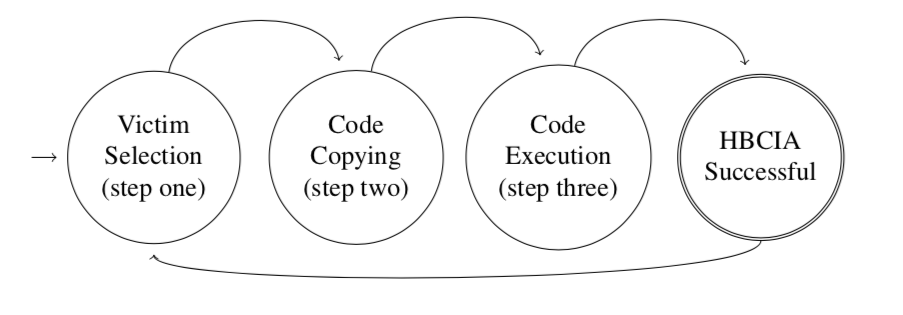
\includegraphics[scale=0.4]{hbcia_3step_algo.png}

\subsection{Code Injection Methods}


\subsubsection{\citetitle{Mitre:2017}}
\textcite{Mitre:2017}

Adversaries may inject code into processes in order to evade process-based defenses as well as possibly elevate privileges. Process injection is a method of executing arbitrary code in the address space of a separate live process. Running code in the context of another process may allow access to the process's memory, system/network resources, and possibly elevated privileges. Execution via process injection may also evade detection from security products since the execution is masked under a legitimate process. 

There are many different ways to inject code into a process, many of which abuse legitimate functionalities. These implementations exist for every major OS but are typically platform specific. 
More sophisticated samples may perform multiple process injections to segment modules and further evade detection, utilizing named pipes or other inter-process communication (IPC) mechanisms as a communication channel. 


\citetitle{Oosthoek:2019}

\textcite{Oosthoek:2019}


\begin{itemize}
\item T1055.001	Dynamic-link Library Injection
\item T1055.002	Portable Executable Injection
\item T1055.003	Thread Execution Hijacking
\item T1055.004	Asynchronous Procedure Call
\item T1055.005	Thread Local Storage
\item T1055.008	Ptrace System Calls
\item T1055.009	Proc Memory
\item T1055.011	Extra Window Memory Injection
\item T1055.012	Process Hollowing
\item T1055.013	Process Doppelgänging
\item T1055.014	VDSO Hijacking
\item T1055.015	ListPlanting
\end{itemize}


\begin{table}[h!]
\centering
\begin{tabular}{ |p{1.2cm}||p{2cm}|p{11.5cm}|  }
  \hline
  \multicolumn{3}{|c|}{PI Mitigation List} \\
  \hline
  ID	& Mitigation & Description \\
  \hline
  M1040	& Behavior Prevention on Endpoint &	Some endpoint security solutions can be configured to block some types of
                                            process injection based on common sequences of behavior that occur during the
                                            injection process. For example, on Windows 10, Attack Surface Reduction (ASR)
                                            rules may prevent Office applications from code injection. [78] \\
  \hline
  M1026 & Privileged Account Management	& Utilize Yama (ex: /proc/sys/kernel/yama/ptrace\_scope) to mitigate ptrace based
                                          process injection by restricting the use of ptrace to privileged users only. Other
                                          mitigation controls involve the deployment of security kernel modules that provide
                                          advanced access control and process restrictions such as SELinux, grsecurity,
                                          and AppArmor. \\
  \hline
\end{tabular}
\label{table: Mitigations}
\end{table}

\begin{table}[h!]
\centering
\begin{tabular}{ |p{1.2cm}||p{2cm}|p{3cm}|p{8cm}|  }
  \hline
  \multicolumn{4}{|c|}{PI Detection List} \\
  \hline
  ID	& Data Source & Data Component & Detects \\
  \hline
   & & & \\
  DS0022 & File & File Metadata & Monitor for contextual data about a file, which may include information such as name,
                                  the content (ex: signature, headers, or data/media), user/ower, permissions, etc. \\
        & & File Modification & Monitor for changes made to files that may inject code into processes in order to evade
                                process-based defenses as well as possibly elevate privileges. \\
  \hline
  DS0011 & Module & Module Load & Monitor DLL/PE file events, specifically creation of these binary files as well as
                                  the loading of DLLs into processes. Look for DLLs that are not recognized or not
                                  normally loaded into a process. \\
  \hline
  DS0009 & Process & OS API Execution & Monitoring Windows API calls indicative of the various types of code injection
                                        may generate a significant amount of data and may not be directly useful for
                                        defense unless collected under specific circumstances for known bad sequences
                                        of calls, since benign use of API functions may be common and difficult to
                                        distinguish from malicious behavior. Windows API calls such as CreateRemoteThread,
                                        SuspendThread/SetThreadContext/ResumeThread, QueueUserAPC/NtQueueApcThread, and
                                        those that can be used to modify memory within another process, such as
                                        VirtualAllocEx/WriteProcessMemory, may be used for this technique.[79] Monitoring
                                        for Linux specific calls such as the ptrace system call should not generate large
                                        amounts of data due to their specialized nature, and can be a very effective
                                        method to detect some of the common process injection methods.[80] [81] [82] [83] \\
        & & Process Access & Monitor for processes being viewed that may inject code into processes in order to
                             evade process-based defenses as well as possibly elevate privileges. \\
        & & Process Metadata & Monitor for process memory inconsistencies, such as checking memory ranges against a
                               known copy of the legitimate module.[84] \\
        & & Process Modification & Monitor for changes made to processes that may inject code into processes in order
                                   to evade process-based defenses as well as possibly elevate privileges. \\
  \hline
\end{tabular}
\label{table: Detection}
\end{table}

\pagebreak

\subsubsection{\citetitle{Hosseini:2017}}
\textcite{Hosseini:2017}

\begin{table}[h!]
\centering
\begin{tabular}{ |p{3.5cm}||p{1.2cm}|p{10cm}|  }
  \hline
  \multicolumn{3}{|c|}{Ten process injection techniques} \\
  \hline
  Name	& ID & Description \\
  \hline
  Classic Dll Injection Via Createremotethread And Load Library
        & T1055 .001
             & The malware writes the path to its malicious dynamic-link
               library (DLL) in the virtual address space of another process,
               and ensures the remote process loads it by creating a remote thread in the target process. \\
  \hline
  Portable Executable (PE) Injection
        & T1055 .002
             & Copy malicious code into an existing open process and cause it to execute (either via a
               small shellcode, or by calling CreateRemoteThread). The malware does not have to drop a
               malicious DLL on the disk; still allocates memory in a host process (e.g. VirtualAllocEx),
               but writes its malicious code by calling WriteProcessMemory. \\
  \hline
  Process Hollowing (A.K.A Process Replacement and Runpe)
        &
             & malware unmaps (hollows out) the legitimate code from memory of the target process, and
               overwrites the memory space of the target process (e.g., svchost.exe) with a malicious executable.\\
  \hline
  Thread Execution Hijacking (A.K.A Suspend Inject and Resume (SIR)
        & T1055 .003
             & After getting a handle to the target thread, the malware puts the thread into suspended mode by
               calling SuspendThread to perform its injection. The malware calls VirtualAllocEx and
               WriteProcessMemory to allocate memory and perform the code injection. Targeting an existing thread
               of a process, during analysis you will probably see calls to CreateToolhelp32Snapshot and
               Thread32First followed by OpenThread. \\
  \hline
  Hook Injection via Setwindowshookex
        &
             & Malicious DLL loaded upon an event getting triggered in a specific thread. This is usually
               done by calling SetWindowsHookEx to install a hook. \\
  \hline
  Injection and Persistence via Registry Modification (E.G. Appinit\_DLLS, AppCertDLLs, IFEO)
        &
             & Appinit\_DLL, AppCertDlls, and IFEO (Image File Execution Options) are all registry keys that
               malware uses for both injection and persistence. \\
  \hline
  APC Injection And Atombombing
        & T1055 .004
             & Use APC to force another thread to execute their custom code by attaching it to the APC
               Queue of the target thread. \\
  \hline
  Extra Window Memory Injection (EWMI) via Setwindowlong
        &
             & Injecting into Explorer tray window’s extra window memory, and has been used a few times
               among malware families such as Gapz and PowerLoader. There is not much room in EWM, so the
               malware writes code into a shared section of explorer.exe, and uses SetWindowLong and
               SendNotifyMessage to have a function pointer to point to the shellcode, and then execute it. \\
  \hline
  Injection Using Shims
        &
             & Shims allow developers to apply fixes to their programs without the need of rewriting code.
               Malware can take advantage of shims to target an executable for both persistence and injection.
               Windows runs the Shim Engine when it loads a binary to check for shimming databases in order
              to apply the appropriate fixes. \\
  \hline
  At Hooking and Inline Hooking (A.K.A Userland Rootkits)
        &
            & Malware changes the import address table. When a legitimate application calls an API located
              in a DLL, the replaced function is executed instead of the original one. \\
  \iffalse
\fi
  \hline
\end{tabular}
\label{table: ProcessInjectionTechniques}
\end{table}

\pagebreak

\href{https://learn.microsoft.com/en-gb/windows/win32/sync/asynchronous-procedure-calls}{MS Asynchronous Procedure Calls}

\href{https://learn.microsoft.com/en-gb/windows/win32/winmsg/about-hooks}{Microsoft Win32 Hooks Overview: hook types and example uses}

\subsection{Deploying Payload into Windows Memory Space}

\textbf{\citetitle{Zhan:2018}}: \textcite{Zhan:2018}

The purpose of this post is to discuss deploying the payload into the memory space of a target process for execution. One can use conventional Win32 API for this task that some of you will already be familiar with, but there’s also the potential to be creative using unconventional approaches. For example, we can use API to perform read and write operations they weren’t originally intended for and that might help evade detection.

There are various ways to deploy and execute a payload, but not all are simple to use. Let’s first focus on the conventional API that despite being relatively easy to detect are still popular among threat actors.
Below is a screenshot of VMMap from sysinternals showing the types of memory allocated for the system I’ll be working on (Windows 10). Some of this memory has the potential to be used for storage of a payload.

\textbf{\citetitle{Dequeker:2023}}: \textcite{Dequeker:2023}

Process injection is a family of malware development techniques allowing an attacker to execute a malicious payload into legitimate addressable memory space of a legitimate process.
These techniques are interesting because the malicious payload is executed by a legitimate process that could be less inspected by a security product such as an EDR.
However, in order to perform this injection, the attacker needs to use specific functions for memory allocation, and use execution primitives to write and execute his payload in the remote process. In standard process injection patterns, these functions are usually the following Win32API: VirtuallAllocEx, WriteProcessMemory and CreateRemoteThread.
 
Security products can use this the mandatory use of this type of functions to detect and fight against process injection by monitoring these API calls. Therefore, in order to keep this type of technique viable, attackers must find other ways to allocate, write and execute memory in a remote process.
This post aims to show an alternate technique allowing execution at an arbitrary memory address on a remote process that can be used to replace the standard CreateRemoteThread call.


\begin{figure}[h]
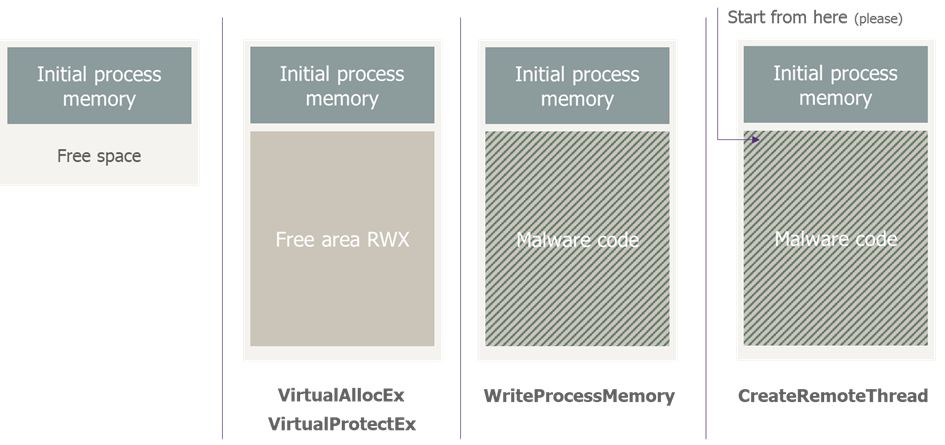
\includegraphics[scale=0.9]{dequeker_standard_process_injection_pattern.png}
\caption{Standard process Injection pattern \autocite{Dequeker:2023}}
\end{figure}
 

\textbf{\citetitle{S12h4ck:2023a}}: \textcite{S12h4ck:2023a}

\href{https://github.com/elddy/Windows-NTAPI-Injector}{GitHub.com Windows-NTAPI-Injector}

\href{https://gist.github.com/WKL-Sec/96e17188e4c159c2cdf7ff2c111130cc#file-local-c}{GitHub.com Injector examples in C}

\textbf{\citetitle{S12h4ck:2023b}}: \textcite{S12h4ck:2023b}

So, picture this: you’re in a digital realm where security is paramount, and there’s an ongoing battle between the good guys and the cyber-criminals. Process injection is like a ninja move in this digital showdown, and these “random RWX memory spaces” are the secret hideouts where the action unfolds.

This C++ code appears to be a Windows application that performs process injection using a specific shellcode into processes that have memory regions marked as PAGE_EXECUTE_READWRITE. Process injection is a technique used in various scenarios, including security research and, unfortunately, malicious activities.


\href{https://www.unknowncheats.me/forum/anti-cheat-bypass/286274-internal-detection-vectors-bypass.html}{internal detection vectors bypass}



\section{Return of the Jedi: EDR}

Review EDR capabilities.  To counter process injection attacts EDR systems can:

\begin{itemize}
\item Static Monitoring of specific DLLs or System Calls: The first level of protection against process injection attack techiques is
  scan processes \ldots
\item Behavioural Analysis: User and entity behaviour analytics (UEBA) are being introduced into XDR tools \ldots
\item Anomaly detection: \autocite{Pek:2016} \ldots
\item Machine Learning techniques: \autocite{Wang:2022}
\end{itemize}


\textbf{\citetitle{Jang:2007}} \textcite{Jang:2007}:

\textbf{\citetitle{Inam:2023}}: \textcite{Inam:2023}.

Auditing, a central pillar of operating system security, has only recently come into its own as an active area of public research. This resurgent interest is due in large part to the notion of data provenance, a technique that iteratively parses audit log entries into a dependency graph that explains the history of system execution. Provenance facilitates precise threat detection and investigation through causal analysis of sophisticated intrusion behaviors. However, the absence of a foundational audit literature, combined with the rapid publication of recent findings, makes it difficult to gain a holistic picture of advancements and open challenges in the area.In this work, we survey and categorize the provenance-based system auditing literature, distilling contributions into a layered taxonomy based on the audit log capture and analysis pipeline. Recognizing that the Reduction Layer remains a key obstacle to the further proliferation of causal analysis technologies, we delve further on this issue by conducting an ambitious independent evaluation of 8 exemplar reduction techniques against the recently-released DARPA Transparent Computing datasets. Our experiments uncover that past approaches frequently prune an overlapping set of activities from audit logs, reducing the synergistic benefits from applying them in tandem; further, we observe an inverse relation between storage efficiency and anomaly detection performance. However, we also observe that log reduction techniques are able to synergize effectively with data compression, potentially reducing log retention costs by multiple orders of magnitude. We conclude by discussing promising future directions for the field.


\subsection{Endpoint Security: EDR}

\textbf{\citetitle{Hayes:2023}} \textcite{Hayes:2023}

Endpoint detection and response (EDR) is a cybersecurity solution that captures all endpoint activity and leverages advanced analytics to provide real-time visibility into the health of all endpoints; detect anomalous activity; alert the information security (Infosec) team to events; and provide remediation suggestions and capabilities to respond, stop an attack in progress or limit its spread.
Endpoint detection and response solutions have the following capabilities:

\begin{itemize}
\item	Endpoint monitoring and event recording
\item	Data search, investigation and threat hunting
\item	Alert triage or suspicious activity validation
\item	Suspicious activity detection
\item	Data analysis
\item	Actionable intelligence to support response
\item	Remediation
\end{itemize}

Managed detection and response (MDR) is endpoint security “as a service.” This  service manages endpoint security technologies for organizations which includes EDR. Service capabilities typically include: :

\begin{itemize}
\item	Continuous monitoring
\item	Threat hunting
\item	Prioritization of threats and alerts
\item	Managed investigation services
\item	Guided response
\item	Managed remediation
\end{itemize}

The main benefit of MDR is that it helps rapidly identify and limit the impact of threats without the need for additional staffing. This is especially important given the global shortage of highly skilled cybersecurity professionals and the related skills gap, particularly as it relates to protection of cloud-based systems and assets.

Extended detection and response (XDR) streamlines security data ingestion, analysis and workflows across an organization’s entire security stack, enhancing visibility around hidden and advanced security threats and unifying the response.

An XDR platform collects and correlates data from across the infrastructure so it can improve threat visibility across the enterprise, accelerate security operations and reduce risk. XDR analyzes, prioritizes and streamlines this data, so it can be delivered to security teams in a normalized format through a single, consolidated console.
XDR platforms typically offer the following capabilities:

\begin{itemize}
\item	Diverse, multi-domain security telemetry
\item	Threat-focused event analysis
\item	Threat detection and prioritization of data fidelity
\item	Data search, investigation and threat hunting across multi-domain telemetry
\item	Response to mitigate and remediate the threat
\end{itemize}

\subsection{What is on offer and where are EDRs failing}

\textbf{\citetitle{Lyles:2022}}: \textcite{Lyles:2022}.

As signature-based malware detection techniques mature, malware authors have been forced to leave fewer footprints on target machines. Malicious activity can be conducted by chaining together benign, built-in functions in subversive ways. Because the functions are native to the host system, attackers can slip under the radar of signature filtering tools such as YARA. To address this challenge, we utilize the Volatility memory forensics framework to measure and characterize typical in-memory behavior, then observe the deviations from normal use that may indicate a compromise. We demonstrate that processes have characteristic memory footprints, and that machine learning models can flag malicious behavior as anomalous.

\textbf{\citetitle{Inam:2023}}: \textcite{Inam:2023}.

Auditing, a central pillar of operating system security, has only recently come into its own as an active area of public research. This resurgent interest is due in large part to the notion of data provenance, a technique that iteratively parses audit log entries into a dependency graph that explains the history of system execution. Provenance facilitates precise threat detection and investigation through causal analysis of sophisticated intrusion behaviors. However, the absence of a foundational audit literature, combined with the rapid publication of recent findings, makes it difficult to gain a holistic picture of advancements and open challenges in the area.In this work, we survey and categorize the provenance-based system auditing literature, distilling contributions into a layered taxonomy based on the audit log capture and analysis pipeline. Recognizing that the Reduction Layer remains a key obstacle to the further proliferation of causal analysis technologies, we delve further on this issue by conducting an ambitious independent evaluation of 8 exemplar reduction techniques against the recently-released DARPA Transparent Computing datasets. Our experiments uncover that past approaches frequently prune an overlapping set of activities from audit logs, reducing the synergistic benefits from applying them in tandem; further, we observe an inverse relation between storage efficiency and anomaly detection performance. However, we also observe that log reduction techniques are able to synergize effectively with data compression, potentially reducing log retention costs by multiple orders of magnitude. We conclude by discussing promising future directions for the field.

\subsection{We're not going to avoid every injection attack}

\textbf{\citetitle{Zengy:2022}}: \textcite{Zengy:2022}.

System auditing provides a low-level view into cyber threats by monitoring system entity interactions. In response to advanced cyber-attacks, one prevalent solution is to apply data provenance analysis on audit records to search for anomalies (anomalous behaviors) or specifications of known attacks. However, existing approaches suffer from several limitations: 1) generating high volumes of false alarms, 2) relying on expert knowledge, or 3) producing coarse-grained detection signals. In this paper, we recognize the structural similarity between threat detection in cybersecurity and recommendation in information retrieval. By mapping security concepts of system entity interactions to recommendation concepts of user-item interactions, we identify cyber threats by predicting the preferences of a system entity on its interactive entities. Furthermore, inspired by the recent advances in modeling high-order connectivity via item side information in the recommendation, we transfer the insight to cyber threat analysis and customize an automated detection system, SHADEWATCHER. It fulfills the potential of high-order information in audit records via graph neural networks to improve detection effectiveness. Besides, we equip SHADEWATCHER with dynamic updates towards better generalization to false alarms. In our evaluation against both real-life and simulated cyber-attack scenarios, SHADEWATCHER shows its advantage in identifying threats with high precision and recall rates. Moreover, SHADEWATCHER is capable of pinpointing threats from nearly a million system entity interactions within seconds.


\subsection{What could detection systems look for}

Looking at memory paging of compromised processes: \citetitle{Pek:2016}, \autocite{Pek:2016}.

Design and implement Membrane, a memory forensics tool to detect code loading behavior by stealthy malware. Instead of trying to detect the code loading itself, we focus on the changes it causes on the memory paging of the Windows operating system. As our method focuses on the anomalies caused by code loading, we are able to detect a wide range of code loading techniques. Our results indicate that we can detect code loading malware behavior with 86.98\% success in most cases, including advanced targeted attacks. Our method is generic enough and hence could significantly raise the bar for attackers to remain stealthy and persist for an extended period of time.

\textbf{\citetitle{Wang:2020}}: \textcite{Wang:2020}.

To subvert recent advances in perimeter and host security, the attacker community has developed and employed various attack vectors to make a malware much stealthier than before to penetrate the target system and prolong its presence. Advanced malware or "stealthy malware" makes use of various techniques to impersonate or abuse benign applications and legitimate system tools to minimize its footprints in the target system. Thus, it is difficult for traditional detection tools, such as malware scanners, to detect it, as the malware normally does not expose its malicious payload in a file and hides its malicious behaviors among the benign behaviors of the processes. In this paper, we present PROVDETECTOR, a provenance-based approach for detecting stealthy malware. Our insight behind the PROVDETECTOR approach is that although stealthy malware attempts to blend into benign processes, the malicious behaviors inevitably interact with the underlying operating system (OS), which will be exposed to and captured by provenance monitoring. Based on this intuition, PROVDETECTOR first employs a novel selection algorithm to identify possible malicious parts in the OS-level provenance data of a process. It then applies a neural embedding and machine learning pipeline to automatically detect any behavior that deviates significantly from normal behaviors. We evaluate our approach on a large provenance dataset from an enterprise network and demonstrate that it achieves very high detection performance of stealthy malware (an average F1 score of 0.974). Further, we conduct thorough interpretability studies to understand the internals of the learned machine learning models.

\textbf{\citetitle{Liu:2023}}: \textcite{Liu:2023}.

Cyber attackers have constantly updated their attack techniques to evade antivirus software detection in recent years. One popular evasion method is to execute malicious code and perform malicious actions only in memory. Malicious programs that use this attack method are called memory-resident malware, with excellent evasion capability, and have posed huge threats to cyber security. Traditional static and dynamic methods are not effective in detecting memory-resident malware. In addition, existing memory forensics detection solutions perform unsatisfactorily in detection rate and depend on massive expert knowledge in memory analysis. This paper proposes MRm-DLDet, a state-of-the-art memory-resident malware detection framework, to overcome these drawbacks. MRm-DLDet first builds a virtual machine environment and captures memory dumps, then creatively processes the memory dumps into RGB images using a pre-processing technique that combines deduplication and ultra-high resolution image cropping, followed by our neural network MRmNet in MRm-DLDet to fully extract high-dimensional features from memory dump files and detect them. MRmNet receives the labeled sub-images of the cropped high-resolution RGB images as input of ResNet-18, which extracts the features of the sub-images. Then trains a network of gated recurrent units with an attention mechanism. Finally, it determines whether a program is memory-resident malware based on the detection results of each sub-image through a specially designed voting layer. We created a high-quality dataset consisting of 2,060 benign and memory-resident programs. In other words, the dataset contains 1,287,500 labeled sub-images cut from the MRm-DLDet transformed ultra-high resolution RGB images. We implement MRm-DLDet for Windows 10, and it performs better than the latest methods, with a detection accuracy of up to 98.34\% . Moreover, we measured the effects of mimicry and adversarial attacks on MRm-DLDet, and the experimental results demonstrated the robustness of MRm-DLDet.


\subsection{It's a bit late, but some feedback to the vendor is in order}

\textbf{\citetitle{Zeng:2021}}: \textcite{Zeng:2021}.

Endpoint monitoring solutions are widely deployed in today's enterprise environments to support advanced attack detection and investigation. These monitors continuously record system-level activities as audit logs and provide deep visibility into security incidents. Unfortunately, to recognize behaviors of interest and detect potential threats, cyber analysts face a semantic gap between low-level audit events and high-level system behaviors. To bridge this gap, existing work largely matches streams of audit logs against a knowledge base of rules that describe behaviors. However, specifying such rules heavily relies on expert knowledge. In this paper, we present WATSON, an automated approach to abstracting behaviors by inferring and aggregating the semantics of audit events. WATSON uncovers the semantics of events through their usage context in audit logs. By extracting behaviors as connected system operations, WATSON then combines event semantics as the representation of behaviors. To reduce analysis workload, WATSON further clusters semantically similar behaviors and distinguishes the representatives for analyst investigation. In our evaluation against both benign and malicious behaviors, WATSON exhibits high accuracy for behavior abstraction. Moreover, WATSON can reduce analysis workload by two orders of magnitude for attack investigation.

\subsection{But will it be good enough}

\textbf{\citetitle{Wang:2022}}: \textcite{Wang:2022}

New malware increasingly adopts novel fileless techniques to evade detection from antivirus programs. Process injection is one of the most popular fileless attack techniques. This technique makes malware more stealthy by writing malicious code into memory space and reusing the name and port of the host process. It is difficult for traditional security software to detect and intercept process injections due to the stealthiness of its behavior. We propose a novel framework called ProcGuard for detecting process injection behaviors. This framework collects sensitive function call information of typical process injection. Then we perform a fine-grained analysis of process injection behavior based on the function call chain characteristics of the program, and we also use the improved RCNN network to enhance API analysis on the tampered memory segments. We combine API analysis with deep learning to determine whether a process injection attack has been executed. We collect a large number of malicious samples with process injection behavior and construct a dataset for evaluating the effectiveness of ProcGuard. The experimental results demonstrate that it achieves an accuracy of 81.58\% with a lower false-positive rate compared to other systems. In addition, we also evaluate the detection time and runtime performance loss metrics of ProcGuard, both of which are improved compared to previous detection tools.

% Section 3 an investigation into the Mockingjay attack and against a recently published paper ``Procguard'' \cite:{Wang:2022} and asks weather this attack method would lickly be caught.
\section{Mockingjay}

The Mockingjay  attack targets trusted and legitimate processes runing on a sytem.  

\textbf{\citetitle{Peixoto:2023}}: \textcite{Peixoto:2023}

\textbf{Why is this technique important?}: It's a new potential security vulnerability. It is a process injection
technique utilised byattackers to deceive robust security products in a corporate environment, such as ``EDRS'' and \textbf{XDRS}.

Process is designed to bypass security controls to gain unauthorised access.

Throughout the blog post, we will delve into various process injection techniques employed by attackers to bypass security controls and gain unauthorized access. We will address the challenges presented by EDRs and XDRs, emphasizing the importance of understanding and mitigating the risks associated with process injection. Additionally, we will share insights gained from our research, including the development of our own process injection technique. We will highlight the capabilities and implications of this technique, shedding light on its effectiveness, potential impact and detection opportunities for defenders.


\section{Figures}

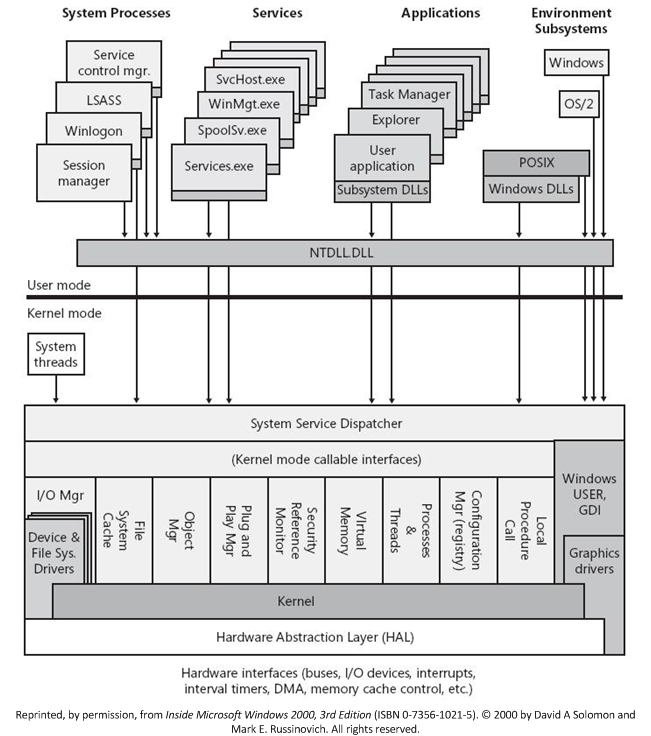
\includegraphics[scale=0.4]{ms_hardware_interfaces.png}

\printbibliography

\end{document}

%%% Local Variables:
%%% mode: latex
%%% TeX-master: t
%%% End: